\chapter{単語の相似関係抽出}
ノード数が等しい二つのグラフG,Hを比較した際、両者の違いが最小となるようにノードを対応させる問題を、\textbf{ノードマッチング問題}という。本研究ではword2vecの出力ベクトル空間上にある任意の二つの形態素集合をそれぞれ、各形態素をノードとみなした重み付き無向グラフと考えて、梅山伸二氏の提案手法\cite{s_umeyama}でノードのマッチング問題を解くことで相似関係を抽出する。

本章では梅山氏の提案手法を説明する。

\section{グラフの同型性問題}
ノード数が等しい二つの重み付き無向グラフG,Hの隣接行列をそれぞれ$A_G$、$A_H$とし、行・列の並び替えを行う転置行列を$P$と表す時、両グラフの違いの大きさを下記の式で定義することができる。
\begin{eqnarray}
  J(P) = ||PA_GP^T-A_H||^2
\end{eqnarray}
$J(P)$の値が最も小さくなる時のノードマッチングが最適なマッチングであり、これを満たす$P$を求める。

\subsection{スペクトル分解}
梅山氏の提案手法で無向グラフのノードマッチングを解くに当たり、まず二つのグラフの隣接行列を固有値分解する。\\
ここからは、下記の二つのグラフを例にして、操作ステップを確認していく。
\begin{figure}[h]
  \centering
  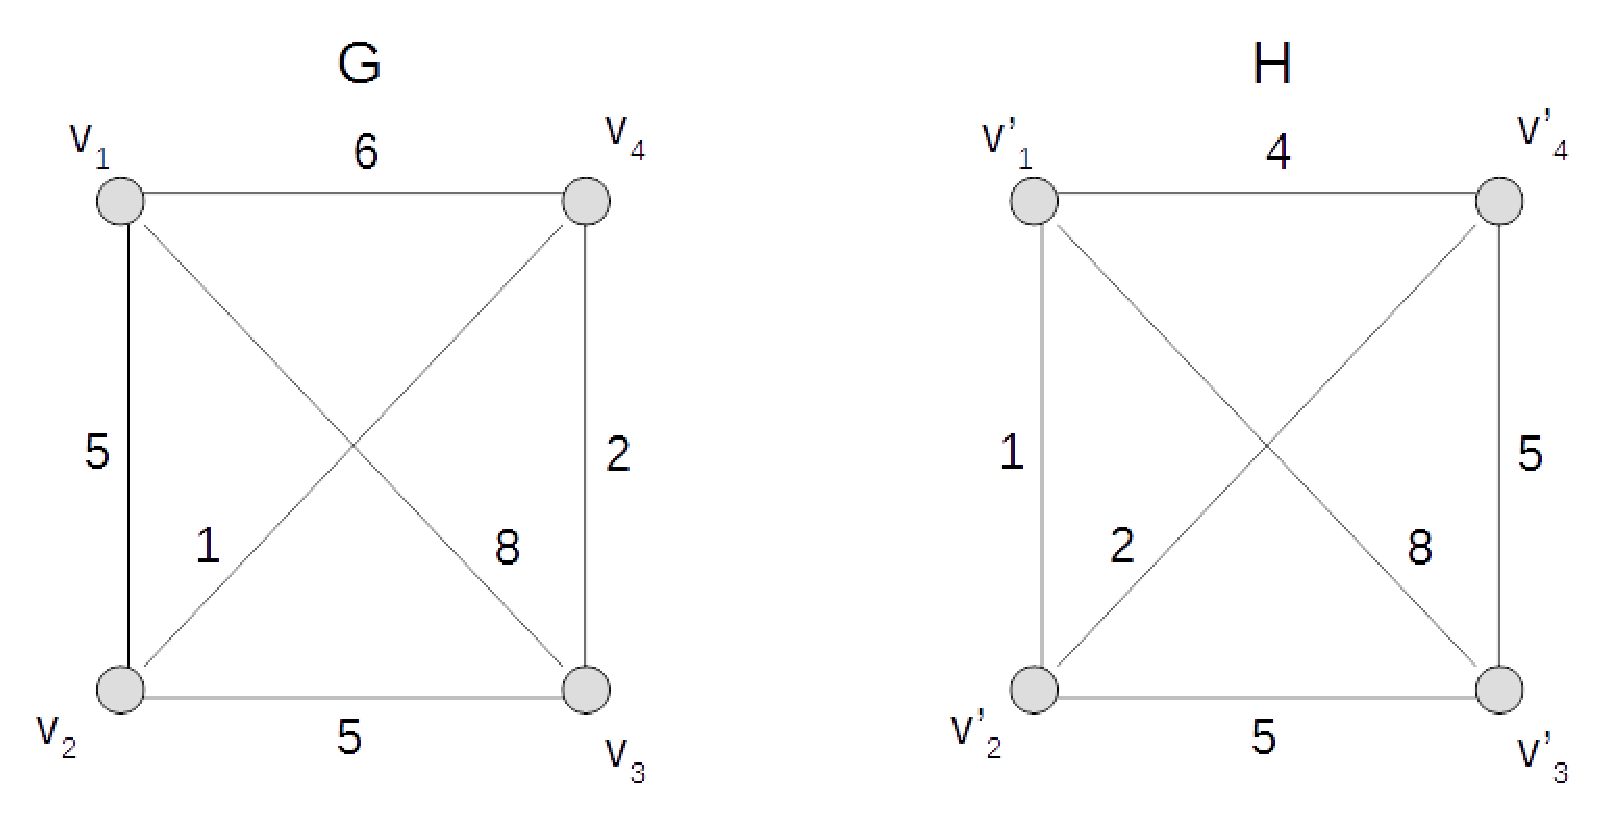
\includegraphics[width=12.5cm]{../images/gh.eps}
  \caption{グラフG、グラフH}
\end{figure}
